%==============================================================
% BAB I  PENDAHULUAN
%==============================================================

\chapter{PENDAHULUAN}

Bab pendahuluan memuat latar belakang atau alasan kuat dilakukannya penelitian,
tujuan, dan hipotesis jika ada.
Di dalam pendahuluan dijelaskan pula perumusan atau pendekatan penyelesaian masalah
dan alasan pemilihan metode yang digunakan.
Bergantung pada proses perumusan masalah penelitian, bagian Kerangka Pikir dan
Hipotesis dapat ditulis di sini, tidak ditulis dalam bab tersendiri.

Paparan tidak berbelit-belit atau dimulai dengan latar belakang yang terlalu umum.
Pernyataan mengenai apa yang diteliti dan apa yang diharapkannya diawali dengan
pemikiran logis.
Tujuan penelitian ditulis di bagian akhir bab ini dengan memilih kata kerja yang
hasilnya dapat diukur dan dilihat, seperti:
\textit{menguraikan, menerangkan, membuktikan, menjajaki, menguji, membuktikan,
atau menerapkan suatu gejala, konsep atau dugaan}, atau bahkan
\textit{membuat suatu prototipe}.
Jangan menggunakan kata kerja mengetahui atau memahami.

Untuk tesis/disertasi dengan pola rangkaian penelitian, dapat dituliskan telaah
pustaka secara umum.
Kebaruan (\textit{novelty}) merupakan hal penting yang harus jelas tersurat atau
tersirat dalam disertasi.
Hal ini berarti penelitian disertasi bukan sekadar mengulang atau mengadaptasi
penelitian yang telah dikerjakan oleh orang lain.
Kebaruan dapat berupa penggunaan metode baru atau pendekatan baru untuk menelaah
suatu permasalahan.


%--------------------------------------------------------------
\section{Latar Belakang}
%--------------------------------------------------------------

Latar Belakang memuat ulasan singkat mengapa penelitian perlu dilakukan.
Uraian dimulai dengan hal yang unik, fakta, masalah, dan pendapat yang mendasari
dilakukannya penelitian.
Di dalamnya diuraikan juga alasan teoretis dan alasan praktis dari perlunya
penelitian dilakukan, dan bagaimana masalah tersebut dapat dipecahkan dan manfaat
dari penyelesaian masalah.


%--------------------------------------------------------------
\section{Rumusan Masalah}
%--------------------------------------------------------------

Berbekalkan latar belakang dan kerangka pikir, masalah yang diteliti dapat
dirumuskan.
Masalah yang dirumuskan harus jelas dan fokus pada kata kunci utama yang unik.
Dalam merumuskan masalah, deskripsi lokasi studi terutama keunikannya sudah
termasuk dalam pertimbangan.
Untuk memperjelas perumusan masalah, dapat juga dibuat beberapa pertanyaan yang
hendak dijawab dalam penelitian itu.
Dalam uraian harus tercakup pendekatan yang digunakan dalam perumusan masalah.
Untuk membantu mengikuti alur pikir secara skematis, dapat juga dibuat bagan alir
kerangka proses dan rumusan masalah serta pencapaian tujuan penelitian.


%--------------------------------------------------------------
\section{Tujuan}
%--------------------------------------------------------------

Pernyataan tujuan penelitian ialah pernyataan singkat dan jelas tentang tujuan
yang akan dicapai sebagai upaya pemecahan masalah maupun memahami gejala
(fenomena) yang dijelaskan dalam latar belakang.
Gunakan kata kerja yang hasilnya dapat diukur.
Bila ada atau memungkinkan, dapat ditulis manfaat atau kegunaan hasil penelitian
bagi kepentingan pengembangan ipteks, pertimbangan dalam mengambil kebijakan,
kepentingan profesi maupun masyarakat pada umumnya.

%--------------------------------------------------------------
% CONTOH GAMBAR
% - Gambar ditempatkan dengan [H] atau [htbp]
% - Caption: di bawah gambar, format "Gambar N Judul"
% - Tanpa bold, tanpa titik dua, hanging indent otomatis
%--------------------------------------------------------------

\begin{figure}[H]
  \centering
  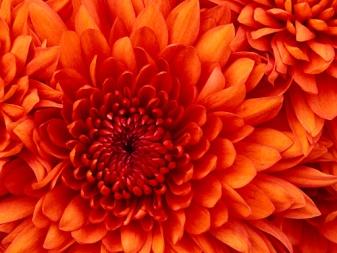
\includegraphics[width=0.5\textwidth]{images/contoh_gambar1}
  \caption{Contoh gambar}
  \label{fig:contoh_gambar1}
\end{figure}


%--------------------------------------------------------------
\section{Manfaat}
%--------------------------------------------------------------

Isi manfaat penelitian menjelaskan kontribusi penelitian terhadap pengembangan
ilmu pengetahuan dan teknologi serta manfaat praktisnya bagi masyarakat
\citep{Widowati2020}.

%--------------------------------------------------------------
% CONTOH TABEL
% Panduan tabel IPB:
% - Caption selalu di atas tabel
% - Format "Tabel N Judul tabel" (tanpa titik dua, tanpa bold)
% - Hanging indent: baris lanjutan rata dengan awal judul
% - Gaya three-line: \toprule, \midrule, \bottomrule (booktabs)
% - Tidak ada garis vertikal
% - Tidak ada garis horizontal internal kecuali setelah header
% - Catatan kaki tabel menggunakan notasi superskrip huruf kecil
%   dan ditulis di bawah tabel dengan \tabularnote atau manual
%--------------------------------------------------------------

\begin{table}[H]
  \caption{Tingkat kekerasan dan kandungan gula buah pisang ambon
           pada suhu simpan yang berbeda dan pemberian putresina}
  \label{tab:pisang_ambon}
  \centering
  \  % Tabel ukuran agak lebih kecil jika konten padat
  \begin{tabular}{lcccccc}
    \toprule
    \multirow{2}{*}{Perlakuan}
      & \multicolumn{6}{c}{Kekerasan buah dan kandungan gula pada hari ke-} \\
    \cmidrule(lr){2-7}
      & \multicolumn{2}{c}{0} & \multicolumn{2}{c}{7} & \multicolumn{2}{c}{14} \\
    \cmidrule(lr){2-3}\cmidrule(lr){4-5}\cmidrule(lr){6-7}
      & Keras$^{\,\mathrm{a}}$ & Gula & Keras$^{\,\mathrm{a}}$ & Gula
      & Keras$^{\,\mathrm{a}}$ & Gula \\
    \midrule
    \multicolumn{7}{l}{\textit{Suhu simpan}} \\
    \quad 15 ºC  & 10.20a & 0.38a & 13.40a & 0.56a & 11.83a & 0.73a \\
    \quad 28 ºC  & 10.64a & 0.55a & 14.22a & 1.82a & 88.43b & 14.41b \\
    \multicolumn{7}{l}{\textit{Putresina}} \\
    \quad Dengan putresina  & 11.07a & 0.53a & 13.23a & 0.87a & 21.19a & 6.98a \\
    \quad Tanpa putresina   & 10.76a & 0.40a & 14.40a & 1.52a & 41.82b & 6.91a \\
    \bottomrule
  \end{tabular}
  % Catatan kaki tabel: rata kiri, ukuran normal, di bawah garis bawah
  \begin{minipage}{\linewidth}
    \vspace{2pt}
    \footnotesize
    $^{\mathrm{a}}$Angka-angka pada kolom yang sama yang diikuti oleh huruf yang
    sama tidak berbeda nyata pada taraf uji 5\% (uji selang berganda Duncan).
  \end{minipage}
\end{table}


%--------------------------------------------------------------
\section{Ruang Lingkup (opsional)}
%--------------------------------------------------------------

Bagian ini menjelaskan batasan dan ruang lingkup penelitian yang dilakukan
agar pembaca dapat memahami cakupan serta keterbatasan studi.

% Contoh gambar dengan judul panjang lebih dari satu baris.
% Baris kedua otomatis dimulai tepat di bawah huruf pertama judul (hanging indent).

\begin{figure}[H]
  \centering
  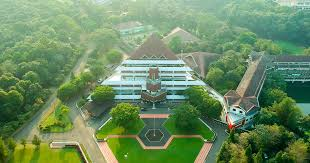
\includegraphics[width=0.7\textwidth]{images/contoh_gambar2}
  \caption{Contoh judul gambar lebih dari satu baris maka baris kedua
           dimulai tepat di bawah huruf pertama judul gambar}
  \label{fig:contoh_gambar2}
\end{figure}


%--------------------------------------------------------------
\section{Hipotesis (opsional)}
%--------------------------------------------------------------

Hipotesis dapat ditulis secara eksplisit atau tersirat sesuai bidang ipteks
yang relevan.
Hipotesis dapat menjadi bagian dari pendahuluan (untuk bidang eksakta atau
kajian eksperimental), atau merupakan bagian akhir dari tinjauan pustaka
(untuk bidang sosial dan ekonomi).
